\documentclass{sigchi}

% Use this section to set the ACM copyright statement (e.g. for
% preprints).  Consult the conference website for the camera-ready
% copyright statement.

% Copyright
%\CopyrightYear{2016}
%\setcopyright{acmcopyright}
%\setcopyright{acmlicensed}
%\setcopyright{rightsretained}
%\setcopyright{usgov}
%\setcopyright{usgovmixed}
%\setcopyright{cagov}
%\setcopyright{cagovmixed}
% DOI
%\doi{http://dx.doi.org/10.475/123_4}
% ISBN
%\isbn{123-4567-24-567/08/06}
%Conference
%\conferenceinfo{CHI'16,}{May 07--12, 2016, San Jose, CA, USA}
%Price
%\acmPrice{\$15.00}

% Use this command to override the default ACM copyright statement
% (e.g. for preprints).  Consult the conference website for the
% camera-ready copyright statement.

%% HOW TO OVERRIDE THE DEFAULT COPYRIGHT STRIP --
%% Please note you need to make sure the copy for your specific
%% license is used here!
% \toappear{
% Permission to make digital or hard copies of all or part of this work
% for personal or classroom use is granted without fee provided that
% copies are not made or distributed for profit or commercial advantage
% and that copies bear this notice and the full citation on the first
% page. Copyrights for components of this work owned by others than ACM
% must be honored. Abstracting with credit is permitted. To copy
% otherwise, or republish, to post on servers or to redistribute to
% lists, requires prior specific permission and/or a fee. Request
% permissions from \href{mailto:Permissions@acm.org}{Permissions@acm.org}. \\
% \emph{CHI '16},  May 07--12, 2016, San Jose, CA, USA \\
% ACM xxx-x-xxxx-xxxx-x/xx/xx\ldots \$15.00 \\
% DOI: \url{http://dx.doi.org/xx.xxxx/xxxxxxx.xxxxxxx}
% }

\toappear{}

% Arabic page numbers for submission.  Remove this line to eliminate
% page numbers for the camera ready copy
\pagenumbering{arabic}

% Load basic packages
\usepackage{balance}       % to better equalize the last page
\usepackage{graphics}      % for EPS, load graphicx instead 
\usepackage[T1]{fontenc}   % for umlauts and other diaeresis
\usepackage{txfonts}
\usepackage{mathptmx}
\usepackage[pdflang={en-US},pdftex]{hyperref}
\usepackage{color}
\usepackage{booktabs}
\usepackage{textcomp}

% Some optional stuff you might like/need.
\usepackage{microtype}        % Improved Tracking and Kerning
% \usepackage[all]{hypcap}    % Fixes bug in hyperref caption linking
\usepackage{ccicons}          % Cite your images correctly!
% \usepackage[utf8]{inputenc} % for a UTF8 editor only

% If you want to use todo notes, marginpars etc. during creation of
% your draft document, you have to enable the "chi_draft" option for
% the document class. To do this, change the very first line to:
% "\documentclass[chi_draft]{sigchi}". You can then place todo notes
% by using the "\todo{...}"  command. Make sure to disable the draft
% option again before submitting your final document.
\usepackage{todonotes}

% Paper metadata (use plain text, for PDF inclusion and later
% re-using, if desired).  Use \emtpyauthor when submitting for review
% so you remain anonymous.
\def\plaintitle{Using statistical quorum to improve utilization of collective attention of democratic communities}
%\def\plainauthor{First Author, Second Author, Third Author,
%  Fourth Author, Fifth Author, Sixth Author}
%\def\emptyauthor{}
%\def\plainkeywords{Authors' choice; of terms; separated; by
%  semicolons; include commas, within terms only; required.}
%\def\plaingeneralterms{Documentation, Standardization}

% llt: Define a global style for URLs, rather that the default one
\makeatletter
\def\url@leostyle{%
  \@ifundefined{selectfont}{
    \def\UrlFont{\sf}
  }{
    \def\UrlFont{\small\bf\ttfamily}
  }}
\makeatother
\urlstyle{leo}

% To make various LaTeX processors do the right thing with page size.
\def\pprw{8.5in}
\def\pprh{11in}
\special{papersize=\pprw,\pprh}
\setlength{\paperwidth}{\pprw}
\setlength{\paperheight}{\pprh}
\setlength{\pdfpagewidth}{\pprw}
\setlength{\pdfpageheight}{\pprh}

% Make sure hyperref comes last of your loaded packages, to give it a
% fighting chance of not being over-written, since its job is to
% redefine many LaTeX commands.
\definecolor{linkColor}{RGB}{6,125,233}
%\hypersetup{%
%  pdftitle={\plaintitle},
%% Use \plainauthor for final version.
%%  pdfauthor={\plainauthor},
%  pdfauthor={\emptyauthor},
%  pdfkeywords={\plainkeywords},
%  pdfdisplaydoctitle=true, % For Accessibility
%  bookmarksnumbered,
%  pdfstartview={FitH},
%  colorlinks,
%  citecolor=black,
%  filecolor=black,
%  linkcolor=black,
%  urlcolor=linkColor,
%  breaklinks=true,
%  hypertexnames=false
%}

% create a shortcut to typeset table headings
% \newcommand\tabhead[1]{\small\textbf{#1}}

% End of preamble. Here it comes the document.
\begin{document}

\title{\plaintitle}

%\numberofauthors{3}
%\author{%
%  \alignauthor{Leave Authors Anonymous\\
%    \affaddr{for Submission}\\
%    \affaddr{City, Country}\\
%    \email{e-mail address}}\\
%  \alignauthor{Leave Authors Anonymous\\
%    \affaddr{for Submission}\\
%    \affaddr{City, Country}\\
%    \email{e-mail address}}\\
%  \alignauthor{Leave Authors Anonymous\\
%    \affaddr{for Submission}\\
%    \affaddr{City, Country}\\
%    \email{e-mail address}}\\
%}

\maketitle

\begin{abstract}
The Achilles heel of many major democracies is the eternal need for sufficient engagement and attention from the community.  While there have been major efforts towards increasing these attributes within the community, we explore a fundamentally different approach: For a fixed level of community attention, how can we optimize the allocation of this attention to maximize productivity?  We propose a novel "statistical quorum", derived using first principles, as one metric the community can use to focus attention, in turn making the entire decision-making process dynamic.  We developed an online system centered around this metric and tested it in a 140-person community that holds weekly councils over the course of 28 weeks.  We found that the community was able to use the online system to simultaneously improve decision-making legitimacy and efficiency.
\end{abstract}

%\category{H.5.m.}{Information Interfaces and Presentation
%  (e.g. HCI)}{Miscellaneous} \category{See
%  \url{http://acm.org/about/class/1998/} for the full list of ACM
%  classifiers. This section is required.}{}{}
%
%\keywords{\plainkeywords}

\section{Introduction}

\section{Features}

\section{Range Voting}

Range voting (also known as score voting) is voting where members of a community express their positions on open proposals by assigning
each a score on a fixed scale, in the context of this paper, between $-1$ and $+1$.
A proposal passes if the average score of all votes on a position is positive.
When multiple competing proposals are being voted on, the one with highest average score wins.

Prior work has shown that this approach generalizes many previous approaches to voting and allows members to express their
positions in a highly informative and precise manner.
We find it especially suitable for a web application because many web users are used to use it when ranking products
and giving other ``five-star'' feedback.
Moreover, if later on a new proposal is added to a set of existing proposals on which voting was already open, only the
new proposal needs to be evaluated by members, as opposed to alternative voting systems where the relative rankings of
each proposal would need reassessing (assuming members use a consistent personal scale when voting).

\subsection{Dynamic Quorum}

%\todo[inline]{Unify terminology: population -> community, voters -> members, item -> proposal, motion -> proposal}

Dynamic quorum uses statistical hypothesis testing to compute the minimum number of required votes needed
to achieve a desired level of confidence before a community adopts an outcome as being truly representative of
its members' positions.
For example, in a community of 100 members, if 20 members vote in full support of a proposal, then we can conclude
with very high confidence that, had all 100 members actually voted, a majority them would support the proposal,
despite in actuality 80 members not having voted.
On the other hand, if 80 members vote but 41 vote in support of the proposal and 39 vote in opposition,
the community cannot yet conclude anything with high confidence.
Hence, the suggested action would be for the community to gather more votes and continue discussion around the proposal.
By utilizing a dynamic quorum, we can direct attention and participation of the community towards contentious proposals,
while reducing attention towards proposals which already have overwhelming support.

\subsubsection{Background}
A population of voters (a community) needs to collectively decide which item (if any) to take action on out of a set of competing items.
In order to democratically take action, the population needs to have a \{simple, super\}-majority of ``yes'' votes on a
winning item, while also demonstrating that the winning item is preferred over all other competing items.
We do not want to poll the entire population, but we do want to be certain (specifically, $99\%$ certain) that
the population does not take undesired actions, which in this case encompasses taking action on an item that is not
supported by a majority of the population and/or taking action on an item that is not clearly preferred over all
other competing alternatives.

\subsubsection{Problem Statement}
We wish to compute the probability that the bias in a population towards voting ``yes'' is greater than some
fraction of the population (e.g., $50\%$ for a simple majority, $67\%$ for a super majority).
In addition, we wish to compute the probability that the bias towards voting ``yes'' on a specific item is greater
than the bias towards voting ``yes'' on all other competing items.

\subsubsection{Assumptions}
We assume that there is a fixed underlying bias in the population that is to be estimated given raw voting data.

Without any votes, we assume that this bias may be any value between $0\%$ and $100\%$ with equal probability.

\subsubsection{Voting}
We allow for range voting where each member of the population may choose any real number in the range $[-1,+1]$ to
represent their vote, with $-1$ representing opposition and $+1$ representing support.
In the theory subsection below, we rescale votes to be in the range $[0,1]$ via the notation $\frac{votes + 1}{2}$.

We allow voters to ``abstain'' from voting.
We treat abstentions as indicating that a voter is removing themselves from the population of voters for an item.
It is important to distinguish an ``abstention'' (removing yourself from the voting population) from voting $0$
(indicating indifference).

\subsubsection{Bayesian Theory}

The commonplace and convenient choice of using the Beta distribution as our prior on the population bias is a
consequence of the Beta distribution's conjugacy with the binomial distribution, a distribution that arises
naturally when considering samples from a finite population.\footnote{To
properly understand the Bayesian approach to parameter estimation, read the following instructive tutorial:
\url{http://www.behind-the-enemy-lines.com/2008/01/are-you-bayesian-or-frequentist-or.html}
The tutorial is very similar to the problem we have at hand.}

After extracting the sufficient statistics from raw votes~---~namely the average score and the number of
abstentions~---~we can adjust the effective population size and corresponding threshold.
In addition, we can calculate the effective number of ``yes'' and ``no'' votes.\footnote{Which one can think
of as the number of Heads and Tails in the aforementioned tutorial.}

Let
\begin{description}
\begin{itemize}
\item[$C = $] $\{X_1,\ldots, X_n\}$, the set of competing motions,
\item[$N = $] population size,
\item[$X_i = $] $\{v_1, \ldots, v_{m_i}\}$, the $m_i$ raw votes for motion $X_i$, excluding ``abstentions'',
\item[$N_i = $] $(N - \textrm{number of abstentions on } X_i)$, the effective population voting on motion $X_i$,
\item[$\alpha_i = $] $\sum\limits_{v \in X_i} \left(\frac{v+1}{2}\right)$, the effective number of ``yes'' votes on motion $X_i$,
\item[$\beta_i = $] $m_i - \alpha_i$, the effective number of ``no'' votes on motion $X_i$,
\item[$K_i = $] $N_i - m_i$, the number of remaining votes yet to be cast on $X_i$,
\item[$p_i = $] true latent population bias towards voting ``yes'' on $X_i$.
\end{itemize}
\end{description}

When we have a single motion open for voting, $C=\{X_1\}$, we simply wish to compute:
\begin{align}\label{eq1}
\Pr(\alpha^*_1 > T_1 \mid X_1),
\end{align}
where
\begin{description}
\begin{itemize}
\item[$\alpha^*_i = $] the total number of ``yes'' votes for $X_i$ if we were to sample the entire population,
\item[$T_i = $] $f \cdot N_i$, for some fraction $f$ corresponding to the type of majority needed for the vote
(e.g. $f=\frac{1}{2}$ for a simple majority).
\end{itemize}
\end{description}
Using the prior $p_1 \mid X_1 \sim \operatorname{Beta}(1+\alpha_1,1+\beta_1)$, corresponding to a uniform prior when
no votes have been cast ($\alpha_1 = \beta_1 = 0$), we can express \eqref{eq1} as:
\begin{align*}
\Pr(\alpha^*_1 > T_1 \mid X_1) &= 1 - \Pr(\alpha^*_1 \leq T_1 \mid X_1),\\
\Pr(\alpha^*_1 \leq T_1 \mid X_1) &= \int_0^1 \Pr(\alpha^*_1 \leq T_1 \mid p_1)\cdot \Pr(p_1 \mid X_1) \mathrm{d}p_1\\
&= \int_0^1 \sum\limits_{i=0}^{V_1} {K_1 \choose i} p_1^{i} {(1-p_1)}^{K_1-i} \\
& \qquad\qquad\quad \times \operatorname{Beta}(p_1; 1+\alpha_1,1+\beta_1) \mathrm{d}p_1,
\end{align*}
where
\begin{description}
\begin{itemize}
\item[$V_i = $] $\lfloor{T_i - \alpha_i}\rfloor$, the maximum number of additional ``yes'' votes allowed such that
$X_i$ would remain below threshold.
\end{itemize}
\end{description}

Hence, we have
\begin{align}\label{eq2}
& \Pr(\alpha^*_1 > T_1 \mid X_1) = \nonumber\\
& 1 - \int_0^1 \sum\limits_{i=0}^{V_1} {K_1 \choose i} p_1^{i} {(1-p_1)}^{K_1-i} \cdot \operatorname{Beta}(p_1; 1+\alpha_1,1+\beta_1) \mathrm{d}p_1
\end{align}

In the scenario where $\mathbf{card}(C) = n > 1$, i.e., there are competing motions, there is additional complexity to
consider.
Without loss of generality, assume that $X_1$ is the most popular motion within $C$.
We now wish to not only compute \eqref{eq1}, but also the probability that $X_1$ is superior to all other
$X_i  \in C, i \neq 1$:

\begin{align}\label{eq3}
\Pr\left(\bigwedge_{i=2}^n (\alpha^*_1 > \alpha^*_i) \mid C\right)
\end{align}

Using the assumption
that votes on motions are independent across motions, which, in the common
scenario where there is a negative covariance between votes on competing
motions, will provide a lower bound on the probability, we can decompose \eqref{eq3} as follows:
\begin{align*}
& \Pr\left(\bigwedge_{i=2}^n (\alpha^*_1 > \alpha^*_i) \mid C\right)\\
=& \prod_{i=2}^n \Pr(\alpha^*_1 > \alpha^*_i \mid C)\\
=& \prod_{i=2}^n \iint\limits_{p_1, p_i} \Pr(\alpha^*_1 > \alpha^*_i \mid p_1, p_i) \cdot \Pr(p_1 \mid X_1) \cdot \Pr(p_i \mid X_i) \mathrm{d}p_i \mathrm{d}p_1\\
=& \prod_{i=2}^n \int_0^1 \int_0^1 \Pr(\alpha^*_1 > \alpha^*_i \mid p_1, p_i) \cdot \operatorname{Beta}(p_1; 1+\alpha_1,1+\beta_1) \\
& \qquad\qquad\qquad \times \operatorname{Beta}(p_i; 1+\alpha_i,1+\beta_i) \mathrm{d}p_i \mathrm{d}p_1\\
\end{align*}
Deriving an expression for $\Pr(\alpha^*_1 > \alpha^*_i \mid p_1, p_i)$, we get:
\begin{align*}
& \Pr(\alpha^*_1 > \alpha^*_i \mid p_1, p_i)\\
=& 1 - \Pr(\alpha^*_1 \leq \alpha^*_i \mid p_1, p_i)\\
=& 1 - \sum\limits_{m=0}^{K_1} \sum\limits_{n=\lceil{v_{1,i}+m}\rceil}^{K_i} {K_1 \choose m} p_1^{m} {(1-p_1)}^{K_1 - m} \cdot {K_i \choose n} p_i^{n} {(1-p_i)}^{K_i-n},
\end{align*}
where
\begin{description}
\begin{itemize}
\item[$v_{i,j} = $] $\alpha_i - \alpha_j$, the number of effective ``yes'' votes $X_i$ leads $X_j$ by.
\end{itemize}
\end{description}

Denoting
\begin{align}\label{eq4}
& \Phi_i(p_1,p_i) {\overset {\underset {\mathrm {def} }{}}{=}} \nonumber\\
& 1 - \sum\limits_{m=0}^{K_1} \sum\limits_{n=\lceil{v_{1,i}+m}\rceil}^{K_i} {K_1 \choose m} p_1^{m} {(1-p_1)}^{K_1 - m} \cdot {K_i \choose n} p_i^{n} {(1-p_i)}^{K_i-n},
\end{align}
we can simplify \eqref{eq3} to:
\begin{align}\label{eq5}
& \Pr\left(\bigwedge_{i=2}^n (\alpha^*_1 > \alpha^*_i) \mid C\right)\nonumber\\
&= \prod_{i=2}^n \int_0^1 \int_0^1 \Phi_i(p_1,p_i) \cdot \operatorname{Beta}(p_1; 1+\alpha_1,1+\beta_1) \nonumber\\
& \qquad\qquad\qquad \times \operatorname{Beta}(p_i; 1+\alpha_i,1+\beta_i) \mathrm{d}p_i \mathrm{d}p_1
\end{align}

We can numerically compute \eqref{eq2} and \eqref{eq5} given raw voting data.
In order to be certain before taking any actions, we would like for the computed credibilities to be $\geq 99\%$.

\begin{figure}[ht]
\centering
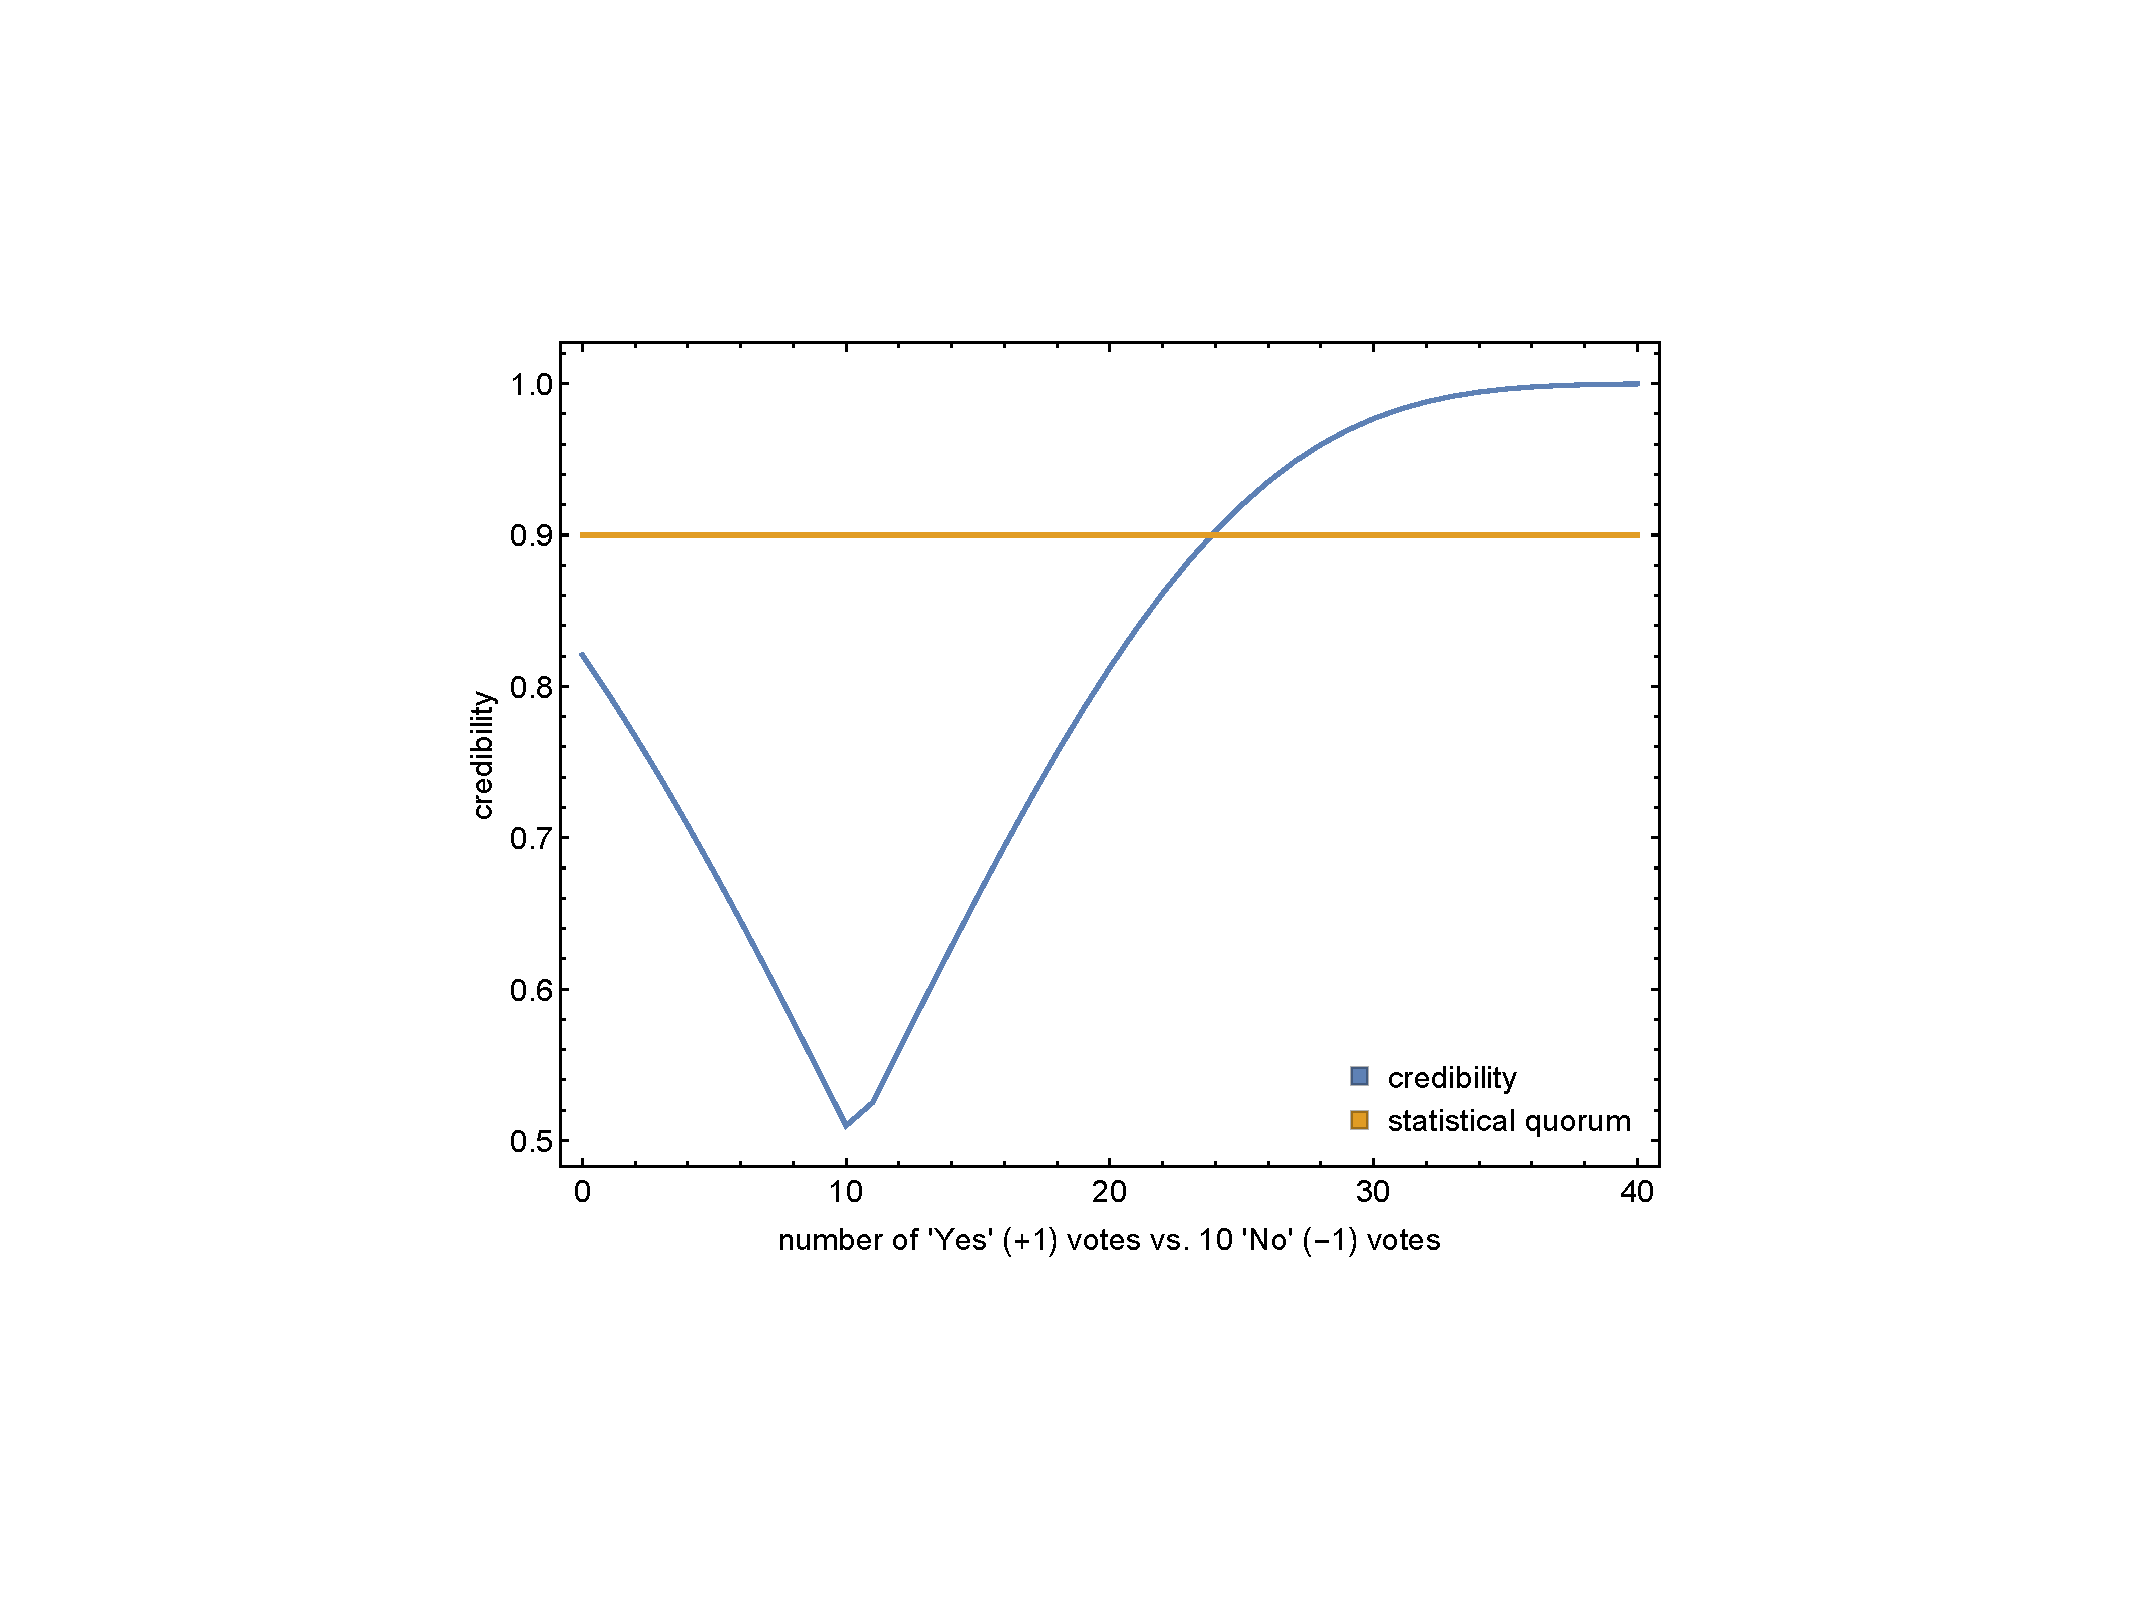
\includegraphics[width=0.5\textwidth]{figures/simple_majority}
\caption{Simple Majority: $\alpha$ vs. $\Pr(\alpha > \frac{1}{2}N)$ for $N=100$, $\beta = 10$.}
\label{simple_majority}
\end{figure}
%Data:
%Curve 1: {{0,0.000299648},{1,0.00213083},{2,0.00817989},{3,0.0224777},{4,0.049512},{5,0.0928927},{6,0.154136},{7,0.232044},{8,0.322859},{9,0.421057},{10,0.520467},{11,0.615358},{12,0.701241},{13,0.775267},{14,0.836245},{15,0.884385},{16,0.920892},{17,0.947532},{18,0.966265},{19,0.978973},{20,0.987296},{21,0.992561},{22,0.99578},{23,0.997682},{24,0.998767},{25,0.999366}}
%Curve 2: {x, 0.99} for all x

\begin{figure}[ht]
\centering
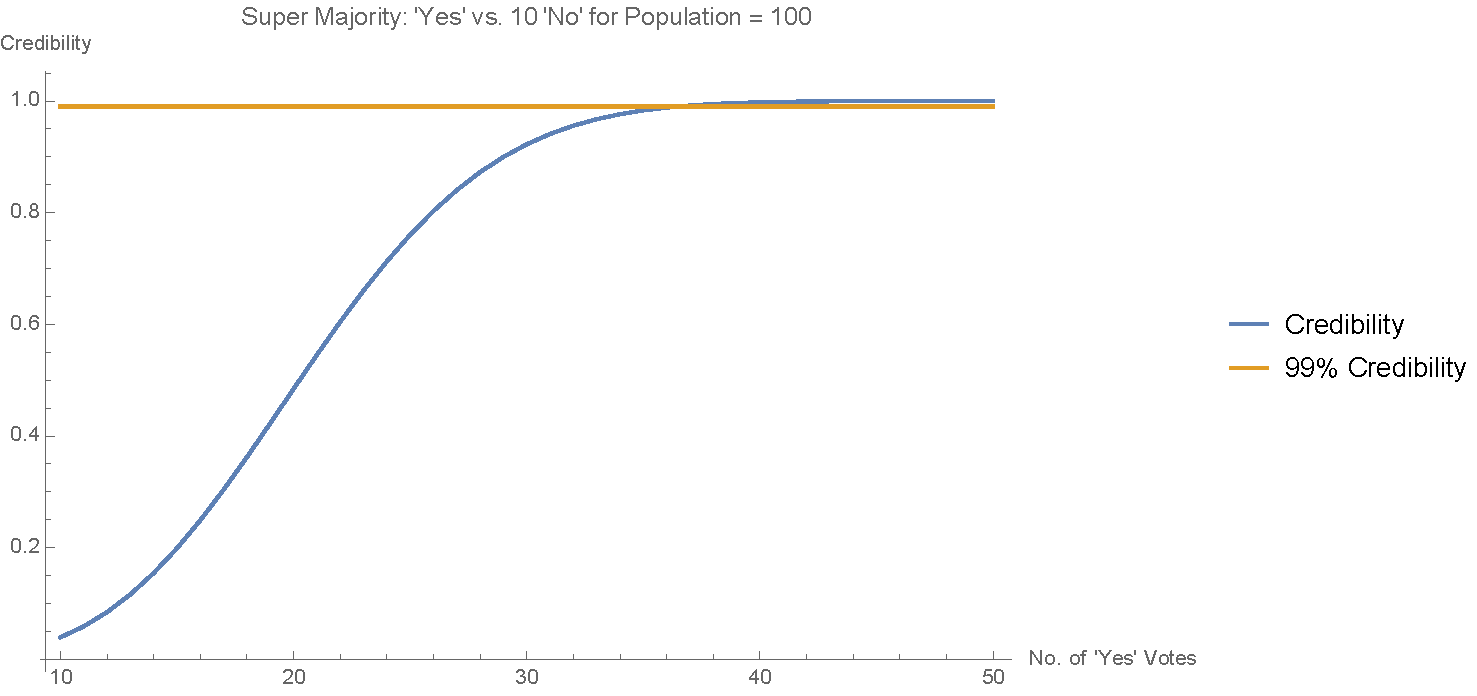
\includegraphics[width=0.5\textwidth]{figures/super_majority}
\caption{Super Majority: $\alpha$ vs. $\Pr(\alpha > \frac{2}{3}N)$ for $N=100$, $\beta = 10$.}
\label{super_majority}
\end{figure}
%Data:
%Curve 1: {{10,0.0395173},{11,0.0591278},{12,0.0846131},{13,0.116407},{14,0.15463},{15,0.199057},{16,0.24911},{17,0.303899},{18,0.362273},{19,0.422909},{20,0.484399},{21,0.545345},{22,0.604445},{23,0.660559},{24,0.712764},{25,0.760382},{26,0.802985},{27,0.840385},{28,0.872612},{29,0.899875},{30,0.922519},{31,0.940987},{32,0.955777},{33,0.967407},{34,0.976384},{35,0.983186},{36,0.988243},{37,0.99193},{38,0.994567},{39,0.996414},{40,0.997682},{41,0.998533},{42,0.999093},{43,0.999452},{44,0.999677},{45,0.999815},{46,0.999896},{47,0.999944},{48,0.99997},{49,0.999985},{50,0.999993}}
%Curve 2: {x, 0.99} for all x

%\todo[inline]{Do we take into the account the distribution of votes? So if you have a very large standard deviation
%we might want to prefer a decision less than some other decision with smaller standard deviation, but maybe
%also smaller (but still positive) average. Is distribution of votes influencing dynamic quorum?}

% REFERENCES FORMAT
% References must be the same font size as other body text.
%\bibliographystyle{sigchi}
%\bibliography{refs}

\end{document}

%%% Local Variables:
%%% mode: latex
%%% TeX-master: t
%%% End:
